\chapter{实验环境}
\section{模型设计}
考虑在具有多种可调度资源的单个服务器上混合执行延迟敏感型任务和批处理任务的问题。智能体执行调度的周期可设置为足够小,以至于在每个时间步骤内,延迟敏感型任务的负载基本不发生变化。通过调度决策开始时到延迟敏感型应用的请求数量,可以预计此段时间步骤内延迟敏感型任务的负载强度。根据预计的负载强度和当前服务器的各类资源利用率(环境状态),智能体选择动作进行资源调度。在当前周期结束后,智能体将收到新的预计负载强度和新的服务器资源利用率。同时,智能体还会收到反映上一个动作质量的奖励信号。

智能体的优化目标是在不违反延迟敏感型任务的服务质量要求的同时,优化服务器的资源利用率。当我们假设批处理任务可以充分利用被分配的资源时,一个相关的且容易量化的优化目标为分配给延迟敏感型任务的资源尽量少。上述假设通常时成立的。

\subsection{隔离技术}
\textbf{计算核心资源}直接影响任务获得的计算速度和并行计算能力。通过Linux系统提供的cgroup,我们可以任意为延迟敏感型任务和批处理任务分配计算核心。实验在英特尔Xeon(R
) E5-2630上进行。该处理器具有10个物理计算核心,20个逻辑计算核心。英特尔的超线程技术使得共用同一个物理计算核心的超线程将共用一二级高速缓存。对于非末级高速缓存的访问目前没有办法进行有效隔离,因此我们将资源分配的粒度设置为分配物理核心以防止批处理任务与延迟敏感型任务在同一物理核心上运行时在一二级高速缓存上产生干扰。\textbf{末级高速缓存}上批处理任务对延迟敏感型任务在延迟敏感型任务高负载强度时产生巨大的干扰。因此隔离任务对末级高速缓存的使用能有效保证延迟敏感型任务在高负载强度时的服务质量。处理器硬件提供20级的缓存分配,为简化问题,我们将缓存分配设置为10级,即资源分配的粒度为末级高速缓存总大小的十分之一。用于控制\textbf{动态随机存储访问带宽}的内存带宽分配技术(MBA)在实验环境的服务器上缺乏硬件支持,因此无法直接控制混合执行任务对动态随机存储器的访问。用于替代内存带宽分配技术,我们通过内存带宽监控技术(MBM)检测每个计算核心产生的动态随机存储访问流量,当批处理任务对动态随机存储访问带宽产生过大压力时,减少分配给批处理任务的计算核心以降低其对动态随机存储的访问。

\subsection{整体架构}
为避免资源调度算法与延迟敏感型程序抢夺资源,资源调度程序将在单独的硬件上运行,并通过与延迟敏感型程序混合执行的一个轻量控制程序监控资源利用和进行资源调度。系统的整体架构如图\ref{fig:overview}所示。

充当资源调度程序的智能体通过与其运行在同一服务器上的控制器与环境交互。当只能体做出动作时,控制器接受智能体的动作,并将其传递至被调度服务器上执行。被调度的服务器上运行的轻量控制器将在指定的时间内取样服务器的资源利用率并返回给调度程序端的控制器。除了执行来自智能体的动作,控制器还将调动负载模拟程序向延迟敏感型任务施加负载并收回此段时间内的服务质量报告。为了获得具有统计学意义的数据,以上施加负载和采样资源利用率的过程都被设定为进行15秒以允许延迟敏感型任务服务足够多的请求。所有搜集到的数据,包括资源利用率报告和服务质量报告,将作为环境状态和计算出的此步骤奖励一起返回给资源调度智能体。

\begin{figure}
  \centering
    \centering
    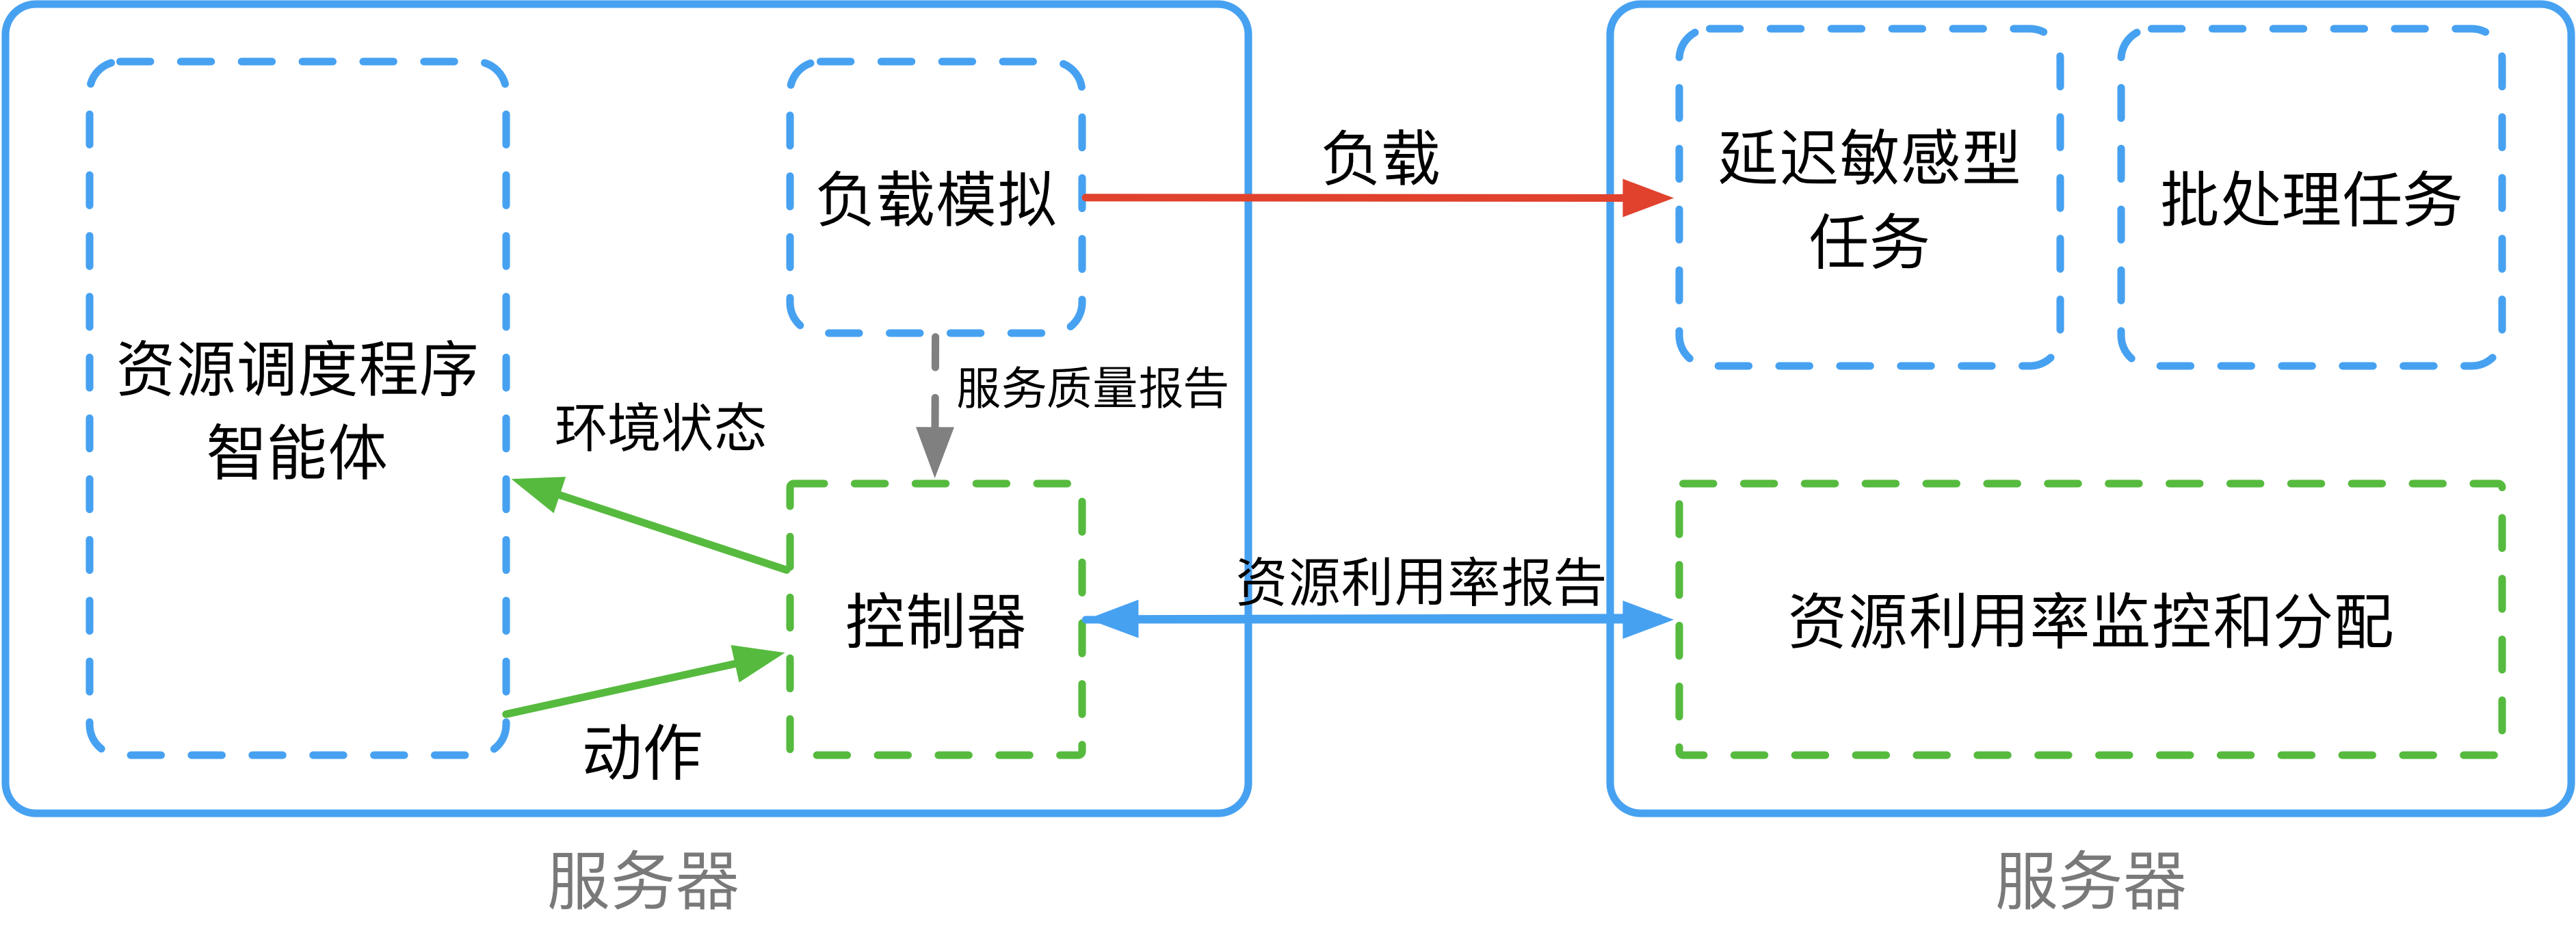
\includegraphics[width=1\linewidth]{exp/overview.png}
    \captionof{figure}{实验系统架构}
    \label{fig:overview}    
\end{figure}


\section{混合执行任务选择}
\subsection{延迟敏感型任务}
数据中心常见的延迟敏感型任务包括社交网络,搜索引擎,软件即服务,在线地图,网页邮箱,机器翻译,在线购物和广告等等。实验中我们选择社交网络作为延迟敏感型任务。

社交网络应用与普通网站服务不同,其更多是一个平台。例如脸书(Facebook)就给用户提供了一个社交平台。社交网络上的大部分数据是由用户(而不是开发者)产生。这些数据由其他用户的行为,或外来资源的变化而引起动态更新,并被推送给用户。正因为如此,社交网络应用包含频繁的后端数据库写入,且写入的数据将在后来推送给用户。

Elgg社交服务引擎是一个基于PHP实现的开源社交网络应用,并被包括澳大利亚政府,新西兰教育部,Wiley出版社,弗罗里达大学在内的机构使用\cite{palit2016demystifying}。Elgg社交服务引擎提供与流行的社交服务脸书提供相似的功能,允许用户在其中建立一个个人好友网络,并在网络中互相分享内容。Elgg社交引擎还包括一个迷你博客Elgg Wire,可用于与其他用户分享文字,图片和视频内容。在Elgg Wire中分享的内容被其他用户可见,类似与脸书中发文上墙的功能。每一个用户都有自己的实时与好友网络共享的信息流,被称为Elgg River。通过Elgg,用户可以实现多种操作,比如发送和接收聊天信息,在Elgg Wire上发送动态,以及接收其他用户最新分享的内容。所有的操作都有AJAX发送和接受简短消息实现,因此Elgg的主要负载都是这些来自AJAX的简短请求。

Elgg的后端通过服务器脚本语言PHP和MySQL数据库实现。脸书的服务器后端相似\cite{nishtala2013scaling},我们还通过Memcached加速数据库访问。为了简化问题,Elgg的网页服务器和后端,包括MySQL和Memcached都运行在同一服务器上,并作为延迟敏感型任务分配资源。

\subsection{批处理任务}
数据中心存在多种批处理任务,例如文件备份,离线图片处理和视频转码压缩等。来自普林斯顿大学的测试程序套装(Princeton Application Repository for Shared-Memory Computer, PARSEC)\cite{bienia11benchmarking}包含了一些典型的数据中心批处理任务。我们选择其中的视频编码测试程序(parsec.x264)作为实验中的批处理任务。

随着存储和网络带宽的增加,网络视频在网络流量中占比显著增加,视频的解码,转码,压缩等任务对于如Youtube的视频网站十分重要。parsec.x264是一个H264/AVC(Advanced Video Coding)的视频编码器,用于将图像有损压缩为一个视频流。与前一代视频编码标准相比,H264添加和改进了位深度(bit depth)和更高分辨率的颜色信息特性,使得其可以以更低比特率输出高质量视频,也因此成为了包括视频会议和视频分发等应用的常用标准。然而H264的优点要考牺牲更多的转码和解码时间得来,因此相比上一代标准,编码和解码H264需要更强的计算能力。

H264编码器和解码器操作在固定的,大小为16乘16的像素块内。多种技术被运用其中以检测和减少数据冗余。其中最重要的技术是运动补偿(Motion Compensation)。动作补偿被应用在连续帧之间以检测每帧图像时间时间上的冗余。动作补偿对最后视频的压缩率有决定性作用,但同时也是压缩视频流时运算量最大的操作。H264编码器输出的帧有三种类型,I类,P类和B类(I-frame, P-frame,B-frame),且每一帧输出对前后一帧输出都有依赖。parsec.x264应用通过流水线模型来并行视频的压缩过程。x264应用并行执行的性质导致其大量的进程间通信,因此共享高速缓存的容量对其性能有较大影响。因为x264的数据输入输出量较大,因此也会对共享高速缓存和动态随机存储器的访问带宽造成较大影响。图\ref{fig:x264}表示了缓存大小对x264的缓存未命中率的影响\cite{bienia2008parsec}。

\begin{figure}
  \centering
    \centering
    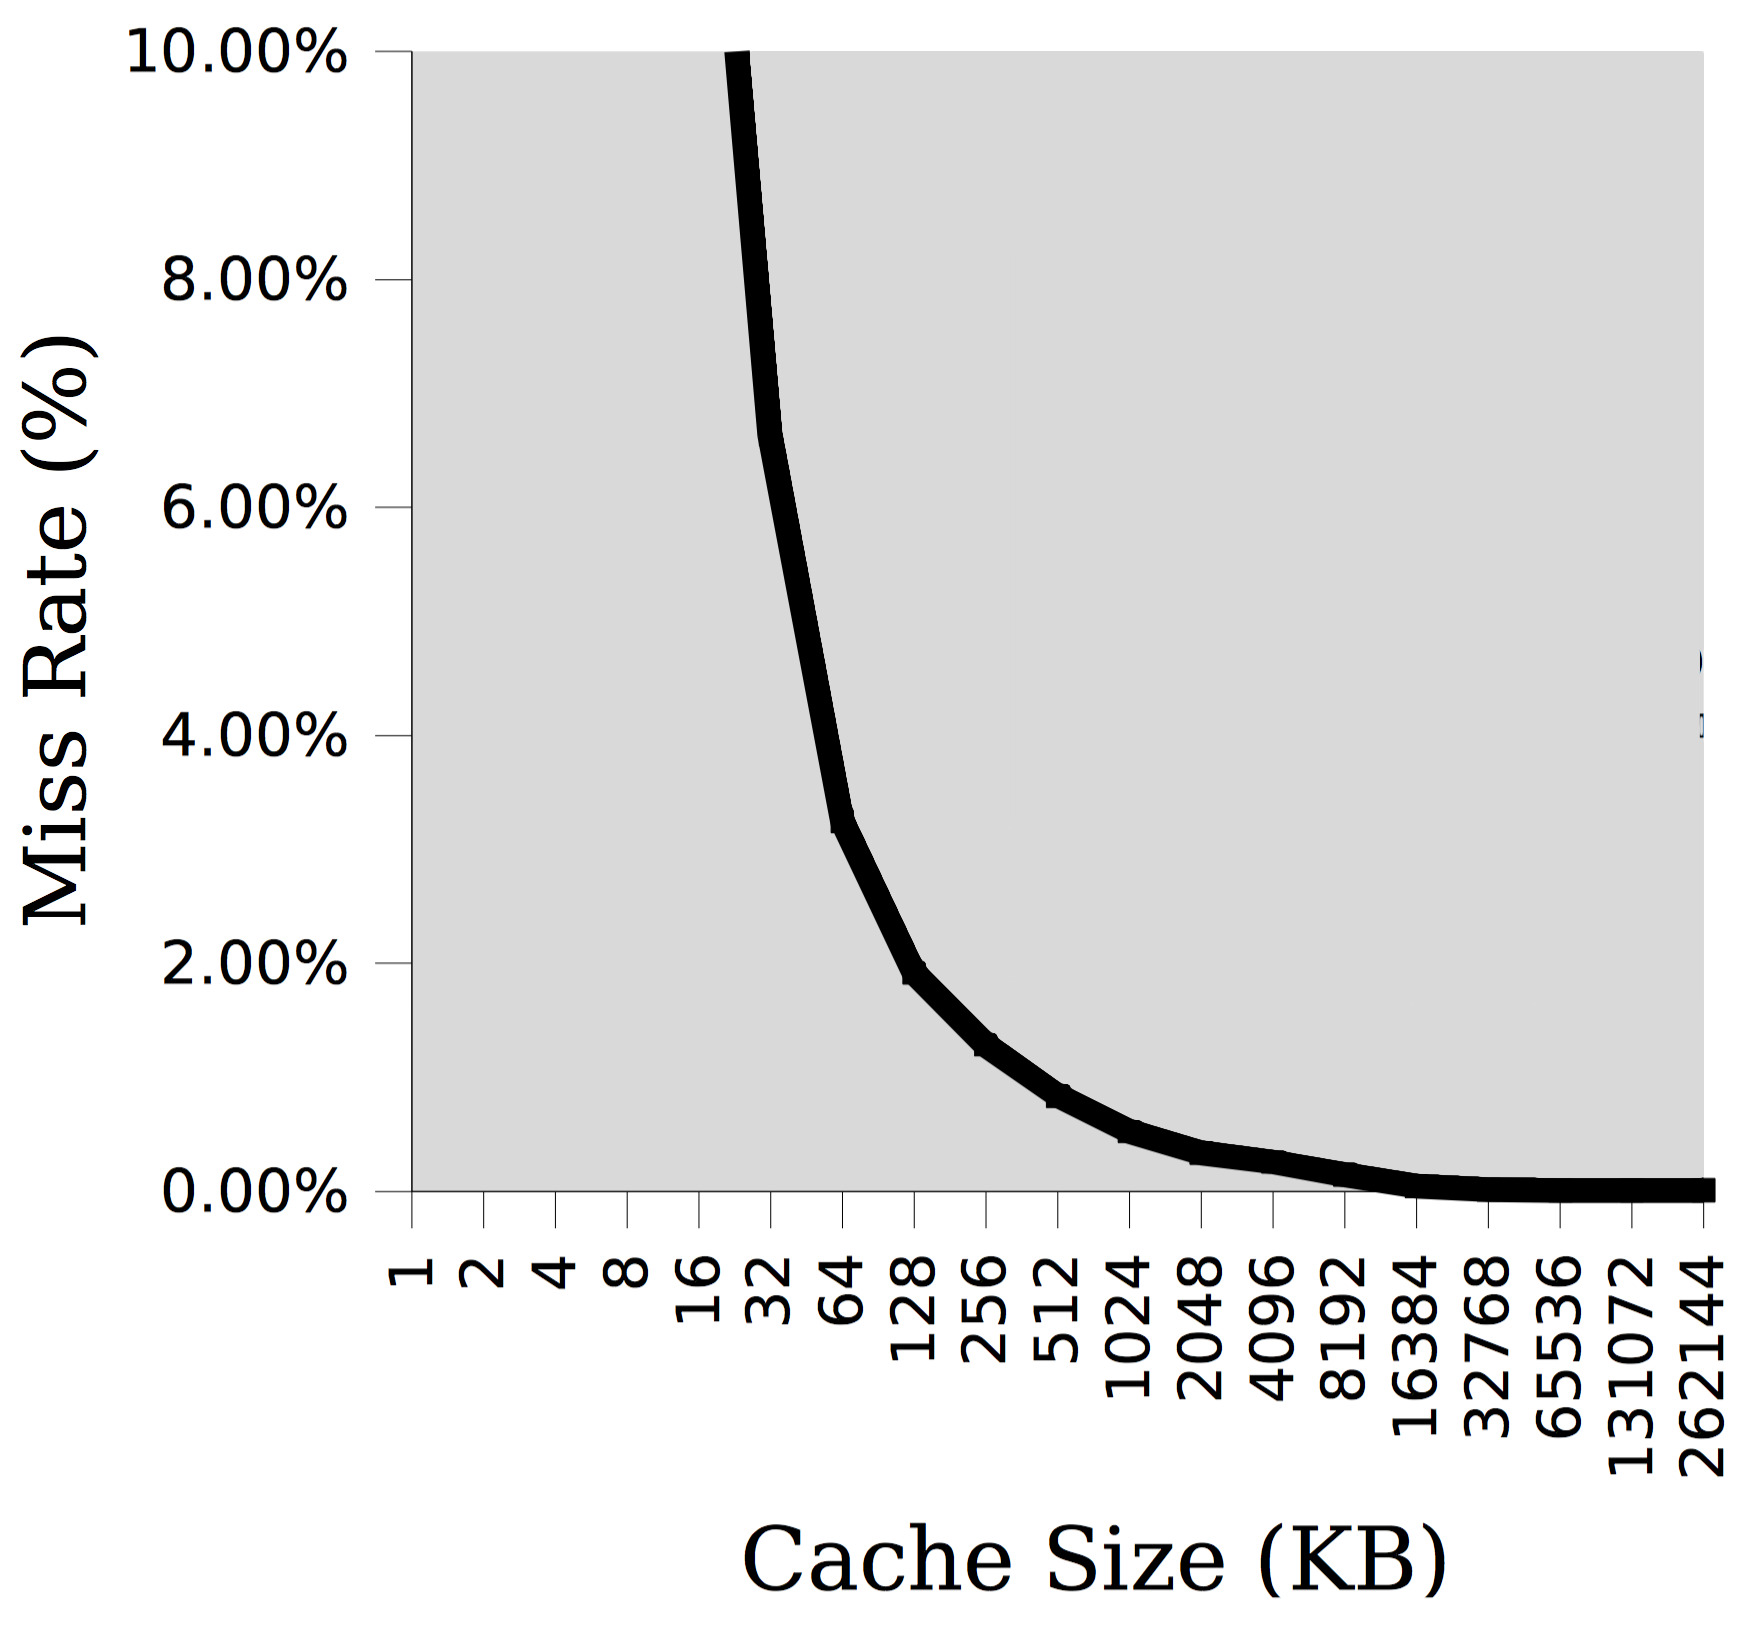
\includegraphics[width=0.5\linewidth]{exp/x264.png}
    \captionof{figure}{x264可用缓存大小与缓存未命中率}
    \label{fig:x264}    
\end{figure}

% x264.png

% \subsection{部署方法}

\section{服务质量测试}

\subsection{测试工具}
我们使用Faban框架来实现Elgg社交引擎的服务质量测试。Faban是一个基于Java的基准测试开发和执行框架,包含两部分Faban驱动框架和Faban Harness。Faban驱动框架提供了API用于快速开发基准测试程序。通过定义测试的操作和各种操作的执行概率,可以快速开发网络应用的基准测试。Faban Harness包含了一个Tomcat实例用于基准测试的自动化部署和执行。在基准测试完成后,Faban Harness将输出各个操作执行情况的统计数据,例如执行测试,相应时间和违反服务质量要求的情况。

\subsection{用户访问模式}
Elgg提供了多种功能,因此用户可以进行多种操作,例如登录登出,添加好友,发送接收消息和分享动态等。考虑到真实用户执行不同操作具有不同频率,且每一个操作与前一个操作具有一定关联,我们通过一个马尔科夫过程(Markov Process)模拟用户的行为,如表\ref{tab:pattern}所示。例如用户登录后有百分之三十的可能性会发动态,百分之五十五的可能性会给好友发送消息。模拟用户每次操作之间的间隔服从指数分布。除用户的主动操作外,应用后台还会固定间隔时间接受消息后刷新用户主页。



通过上述方式模拟用户的操作,从服务器来看,模拟用户总体的产生的各个操作的比例如表\ref{tab:mix}所示。对于Elgg社交应用引擎表的各个操作,其服务质量被定义为一段时间内所有该操作的响应时间的九十分位点。\ref{tab:mix}同时还规定的各个操作的服务质量要求。对于注册,登录和退出等用户不频繁使用的的操作,我们设置了较低的服务质量要求。

\begin{table}[!htp]
  \centering
  \captionof{table}{模拟用户总体访问模式}\label{tab:mix}
  \begin{tabular}{@{}lcc@{}} \toprule
    操作 & 占比 & 服务质量要求\\ 
    \midrule
    注册 & 0.5 & 6 \\
    登录 & 2.5 & 6 \\
    退出 & 2.5 & 6 \\
    首页 & 5 & 2 \\
    动态 & 20 & 2 \\
    好友 & 10 & 2 \\
    发消息 & 17 & 2 \\
    收消息 & 17 & 2 \\
    刷新主页 & 25.5 & 2\\
    \bottomrule
  \end{tabular}  
\end{table}


